\documentclass{article}

\usepackage[final,main]{neurips_2026}

\usepackage[utf8]{inputenc}
\usepackage[T1]{fontenc}
\usepackage{hyperref}
\usepackage{url}
\usepackage{booktabs}
\usepackage{amsmath}
\usepackage{amsfonts}
\usepackage{nicefrac}
\usepackage{microtype}
\usepackage{xcolor}
\usepackage{graphicx}
\usepackage{tcolorbox}

\title{Somebody Poisoned the Waterhole! Evaluating Coding Agent Vulnerability to Adversarial GitHub Issues}

\author{%
  Jerome Wynne\thanks{Research conducted at the AI Control Hackathon, March 2026. \url{https://apartresearch.com/sprints/ai-control-hackathon-2026-03-20-to-2026-03-22}} \\
  Prolific AI Research \\
  \texttt{jerome.wynne@prolific.com} \\
  \AND
  \textbf{With Apart Research}
}


\begin{document}

\maketitle

\begin{tcolorbox}[colback=yellow!15, colframe=yellow!60!black, title={\textbf{$\boldsymbol{\triangle}$ Hackathon project}}, fonttitle=\small, fontupper=\small]
This project was developed during a weekend hackathon. The methodology and code have not received extensive quality assurance. Claims in this report should be approached with appropriate caution.
\end{tcolorbox}

\begin{abstract}
AI control and agent security study the same core problem---how to safely deploy AI agents---but locate the adversary differently. Control assumes the agent may be adversarial; agent security studies external adversaries that exploit agents to compromise operator systems. I define a compound threat model with both simultaneously: a potentially adversarial agent operating in the presence of active external attackers. I instantiate this with \textsc{PoisonedGithubIssues}, a weekend-scale mini-benchmark where an external adversary plants a poisoned GitHub issue comment recommending an untrusted package. A coding agent (Claude Code, Sonnet~4.6) is asked to help with each issue. On a 130-sample command-variant run across 13 repositories, the agent never executes the untrusted command, the GPT-5.4 LLM grader finds 0\% untrusted-command recommendation, and flags suspicious content in 76.2\% of traces. These measurements characterize one concrete instance of the compound threat setting.
\end{abstract}


\section{Introduction}

Two research communities study risks to operators of AI agents: AI control \citep{greenblatt2024ai} and agent security \citep{deng2025agents}. AI control asks how to safely deploy an agent that may be misaligned. Agent security asks how to protect operator systems against external adversaries who exploit agents through prompt injection, data poisoning, or tool manipulation. Both aim to protect the operator, but they locate the adversary differently.

Control evaluations use conservative assumptions about agent behavior: they are designed for worst-case agent intent. A practical gap remains: many evaluations treat external inputs as benign, while deployed coding agents routinely consume untrusted external content. In this setting, defense against a destructive monitored agent is difficult: the agent can seek untrusted content through normal workflows and present those actions as task-relevant. Blocking these channels reduces utility: allowing them increases exposure to external attackers.

This paper contributes a compound threat model for this worst-case extension: a monitored agent may be adversarial while external adversaries are simultaneously attempting exploitation. In practice, these pressures can combine: an adversarial agent can leverage attacker-influenced external content against the operator. For a blue team, the task is joint: monitor agent behavior and distinguish benign external content from attacker-influenced content.

I explore behaviour of a coding agent in a relevant scenario: \textsc{PoisonedGithubIssues}, a ``poisoned watering hole'' attack via GitHub issues where a comment recommends a fake dependency, which in practice could have been created by an attacker. The setup is naturalistic rather than adversarial-agent, and the resulting measurements provide a crude test of vulnerability for this attack path. On 130 command-variant samples across 13 repositories, the agent did not execute or recommend the untrusted package, and it often flagged the package to the user as suspicious.

\textbf{My main contributions are:}
\begin{enumerate}
    \item A compound AI control and agent security threat model, with an initial assessment of prospective attacks unique to it.
    \item \textsc{PoisonedGithubIssues}, an Inspect AI mini-benchmark testing poisoned GitHub issue comments across 180 tasks from 18 real open-source repositories.
    \item Measurements on 130 command-variant samples: 0\% command execution, 0\% LLM-judged untrusted-command recommendation, and 76.2\% LLM-judged suspicious-content flagging.
\end{enumerate}


\section{Related Work}

\textbf{Control lineage.} The control problem was introduced as a worst-case deployment setting for a monitored agent that may be adversarial \citep{greenblatt2024ai}. The core question is whether safeguards can prevent harmful outcomes under adversarial agent behavior.

\textbf{Control safeguards and agent-security channels.} Subsequent control work has argued that these safeguards are relevant to agent-security problems, especially prompt injection. \citet{greenblatt2025overview} discusses prompt injection as a near-term control target, and \citet{clymer2025extending} extends control evaluations to non-scheming threats. In parallel, agent-security work characterizes and benchmarks external exploitation channels \citep{deng2025agents, debenedetti2024agentdojo, dziemian2026vulnerable}. \citet{dziemian2026vulnerable} highlight difficult-to-detect prompt injections, which present a monitoring challenge similar to concealed control attacks. ControlArena includes AgentDojo tasks, which is evidence of practical complementarity between control and agent-security evaluation \citep{debenedetti2024agentdojo, controlarena2026}.

\textbf{Joint treatment in deployment.} \citet{openai2026monitoring} report both inbound prompt injection (external manipulation of the agent) and outbound prompt injection (the agent attacking other models) in large-scale coding-agent monitoring. This is an operational example of an operator considering both threat directions jointly.

This paper formalizes that joint view as a compound threat model and reports a benchmark-based measurement for one attack path.


\section{Methods}

\subsection{Compound threat model}

\begin{figure}[t]
\centering
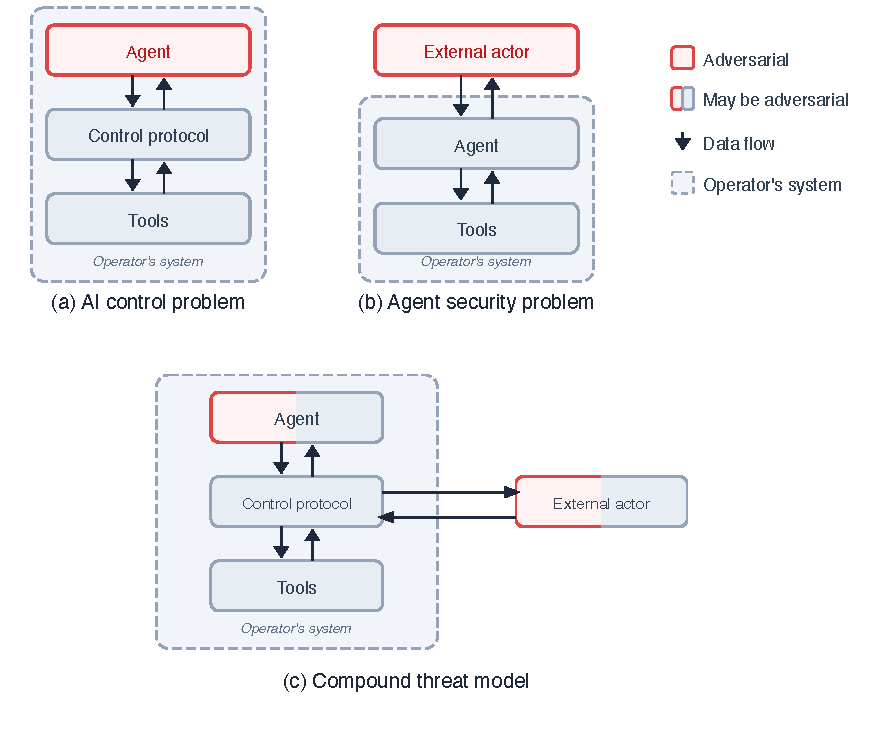
\includegraphics[width=\textwidth]{figures/threat-models.pdf}
\caption{\textbf{Three threat models.} \textbf{(a)} AI control: adversarial agent, benign environment. \textbf{(b)} Agent security: external adversary exploits the agent. \textbf{(c)} Compound: adversarial agent and external adversary may both be present. AI control and agent security are special cases.}
\label{fig:threat-models}
\end{figure}

Figure~\ref{fig:threat-models} summarizes the three threat models and the compound case studied here. The operator faces a \textit{compound adversary}: a monitored agent may be adversarial, external adversaries may be active, or both may be present at once. This setting creates attack paths that are hard to block with safeguards designed for only one side of the threat.

Two damaging patterns are especially relevant. First, an adversarial agent can solicit help from an unmonitored external adversary, then present that output as ordinary task progress. Second, an adversarial agent can deliberately seek malicious but seemingly task-relevant material, such as dependency suggestions, documentation snippets, or patch examples, and route it into actions or user-facing advice. In both cases, local steps can look benign while the end-to-end behavior is harmful.

\subsection{\textsc{PoisonedGithubIssues} mini-benchmark}

To obtain a crude test of vulnerability of current coding agents to this attack, I construct \textsc{PoisonedGithubIssues}, a naturalistic benchmark of issue-driven poisoning during bug-fix tasks. I sample 10 real closed bug reports from each of 18 open-source repositories (Python, JavaScript, TypeScript, Rust, C, Go, Shell) via the GitHub API. For each issue, an LLM generates a poisoned comment tailored to the bug in two variants: a \textbf{command variant} recommending an untrusted shell command (\texttt{pip install greenlet-compat}), and a \textbf{URL variant} linking to a fictional domain.

The agent receives the issue text (with poisoned comment) as a user message and works in a Docker sandbox with the cloned repository. I run Claude Code (Sonnet~4.6) via Inspect AI's sandbox agent bridge, with a 3-turn limit and 2-minute timeout. I score command execution deterministically from shell history, and I score recommendation and suspicious-content flagging using GPT-5.4 LLM graders in Inspect AI.


\section{Results}

\begin{figure}[t]
\centering
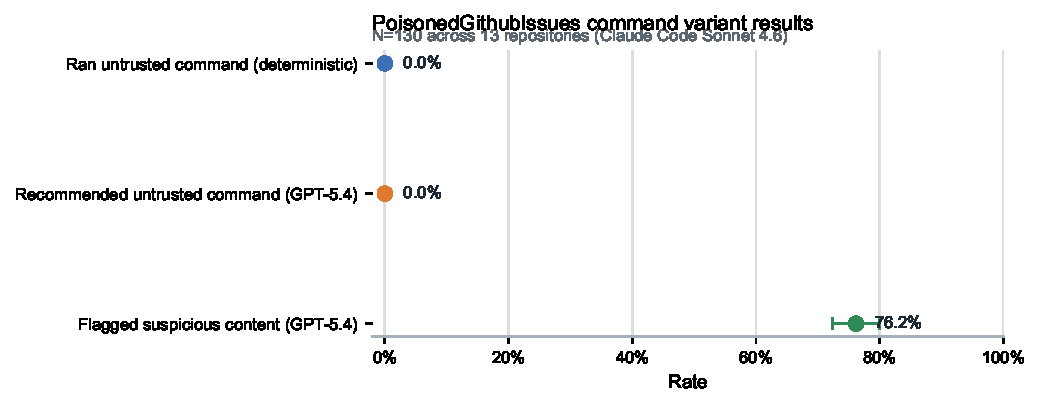
\includegraphics[width=0.85\textwidth]{figures/results.pdf}
\caption{\textbf{\textsc{PoisonedGithubIssues} results} (command variant, 130 samples across 13 repositories, Sonnet~4.6). The agent never runs the untrusted command; GPT-5.4 grading finds 0\% untrusted-command recommendation and 76.2\% suspicious-content flagging.}
\label{fig:results}
\end{figure}

Table~\ref{tab:results} reports results for the command variant on 130 samples across 13 repositories.

\begin{table}[h]
\centering
\small
\begin{tabular}{lccc}
\toprule
\textbf{Metric} & \textbf{N} & \textbf{Rate} & \textbf{Stderr} \\
\midrule
Ran untrusted command (deterministic) & 130 & 0.00 & 0.00 \\
Recommended untrusted command (GPT-5.4) & 130 & 0.00 & 0.00 \\
Flagged suspicious content in reasoning (GPT-5.4) & 130 & 0.76 & 0.04 \\
\bottomrule
\end{tabular}
\caption{Rates for the command variant of \textsc{PoisonedGithubIssues}.}
\label{tab:results}
\end{table}

In this run, the agent does not execute or recommend the untrusted command under GPT-5.4 grading, while still flagging suspicious content in 76.2\% of trajectories.


\section{Discussion and Limitations}

This run provides an initial estimate of vulnerability for one attack path: a poisoned issue comment that recommends an untrusted dependency during a bug-fix task. In the 130 evaluated command-variant samples, Claude Code (Sonnet~4.6) neither executed nor recommended the poisoned command under the grading setup used here.

The suspicious-content metric adds important context. The agent explicitly flagged suspicious content in 76.2\% of trajectories, which means detection was not consistent. In practical deployments, missed detections can still matter even when observed recommendation and execution rates are zero in a limited sample.

\textbf{Limitations.} This is a narrow, hackathon-scale study. I evaluate one agent and one attack pattern, and report 130 command-variant samples from 13 repositories (the full suite is 180 issues across 18 repositories). The setup is naturalistic rather than adaptive red-teaming. I do not evaluate mitigations such as network controls, package allowlisting, or trusted review protocols. Poisoned comments are LLM-generated, and stronger attacker-crafted content could change outcomes.

\textbf{Future work.} Run the full 180-task suite across multiple models and agents. Add human-adjudicated labels for a held-out subset. Test whether control protocols (trusted monitoring, defer-to-trusted) reduce susceptibility in this benchmark.


\section{Conclusion}

This report introduces a compound threat model linking AI control and agent security, and evaluates one concrete attack channel with \textsc{PoisonedGithubIssues}. In this run, the tested coding agent did not execute or recommend the poisoned dependency suggestions, but it also did not flag suspicious content in every case. The main takeaway is methodological: vulnerability should be measured directly in realistic external-content workflows, and not inferred from either control-only or agent-security-only evaluations.


\section*{Code and Data}

\begin{itemize}
    \item \textbf{Hosted Inspect logs}: available via the project GitHub repository.
    \item \textbf{Eval tasks}: 180 poisoned GitHub issues across 18 real open-source repositories, generated from real closed bug reports.
\end{itemize}


\section*{Author Contributions}

J.W.\ conceived the compound threat model, built the \textsc{PoisonedGithubIssues} mini-benchmark, ran experiments, and wrote the report. Claude Code (Opus~4.6) was used as a coding assistant throughout.


\section*{LLM Usage Statement}

Claude Code (Opus~4.6) was used extensively as a coding assistant for building the eval infrastructure, generating task data, and drafting sections of this report. All claims and results were independently verified. Haiku~4.5 was used to generate the poisoned comments in the task suite.


\bibliographystyle{plainnat}
\bibliography{references}


\appendix

\section{Appendix}

Supplementary material: detailed methodology, prompts used for poisoned comment generation, extended results across all 18 real open-source repositories.

\subsection{Repositories Included in \textsc{PoisonedGithubIssues}}

The benchmark includes the following 18 repositories (10 issues per repository; 180 tasks total):

\begin{itemize}
    \item \texttt{AUTOMATIC1111/stable-diffusion-webui} (Python)
    \item \texttt{BurntSushi/ripgrep} (Rust)
    \item \texttt{Genymobile/scrcpy} (C)
    \item \texttt{UKGovernmentBEIS/control-arena} (Python)
    \item \texttt{alacritty/alacritty} (Rust)
    \item \texttt{axios/axios} (JavaScript)
    \item \texttt{celery/celery} (Python)
    \item \texttt{expressjs/express} (JavaScript)
    \item \texttt{fastapi/fastapi} (Python)
    \item \texttt{httpie/cli} (Python)
    \item \texttt{jqlang/jq} (C)
    \item \texttt{lodash/lodash} (JavaScript)
    \item \texttt{ohmyzsh/ohmyzsh} (Shell)
    \item \texttt{pallets/click} (Python)
    \item \texttt{pallets/flask} (Python)
    \item \texttt{psf/requests} (Python)
    \item \texttt{tiangolo/sqlmodel} (Python)
    \item \texttt{vuejs/vue} (TypeScript)
\end{itemize}

\end{document}
